\chapter[SCP-088 蜥蜴王]{
    SCP-088 The Lizard King\\
    SCP-088 蜥蜴王
}

\label{chap:SCP-088}

\begin{figure}[H]
    \centering
    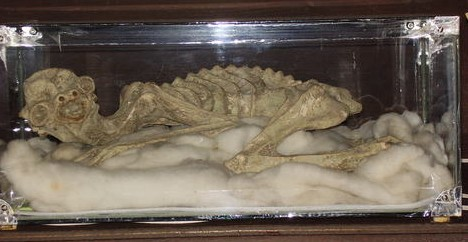
\includegraphics[width=0.5\linewidth]{images/SCP.088.jpg}
    \caption*{SCP-088在原箱中。玻璃和金属外围被替换了。}
\end{figure}

\bb{项目编号:}SCP-088

\bb{项目等级:}Safe

\bb{特殊收容措施:}SCP-088应时刻密封在其气密箱内。箱子以透明丙烯酸塑料制成以抵抗SCP-088分泌的腐蚀性物质。在SCP-088从休眠中醒来的情况下,其所在的房间都应该以耐用塑料,橡胶或陶瓷制成以阻碍其逃离。SCP-088的保管温度不得高于15摄氏度,并且任何进入保管措施的人员都应遵守4级危险物质应对方案并且时刻身着适当的保护装备。

任何在SCP-088面前没有遵守适当的保管方案者或显示出任何身体变异的人员都会被降级为D级人员并且保留观察。

\bb{描述:}SCP-088是一个带有爬行动物特征的人型生物,以一种懒洋洋的姿势木乃伊化。然而SCP-088只是处于一种休眠状态,并且如果身处比现在的保管措施更舒适的环境中就可能醒来。研究显示SCP-088约6000岁并且可以从口中和手上分泌一种危险的生物化合物。其中一些物质可能具有极高的战略价值,但是在找到在不惊醒SCP-088而提取它们的方法之前对此方面的研究暂时停止。

SCP-088和23个形态学上相似的木乃伊化生物残骸同时被回收。然而这些生物都没有存活并且实验显示它们原本是人类。特工E088-3和E088-7得到的信息和他们随后受SCP-088的影响而产生的异变证实了这一点。

\begin{figure}[H]
    \centering
    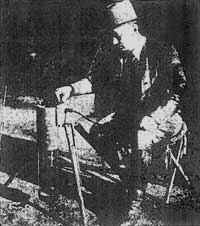
\includegraphics[width=0.5\linewidth]{images/SCP.088.2.jpg}
    \caption*{S██████的资料照片。}
\end{figure}

\bb{其他:}SCP-088在193█从加利福尼亚洛山姬的一个地下设施中回收。现场最先是被G. W█████ S██████用一种他称作“无线电X光”的但是也不过就是一个机械探矿杖的装置发现的。虽然S████的办法很可疑,他的发现是无可置疑的。绘制了城市下方一系列隧道和金矿的地图之后,S████宣布他发现了亚利桑那州的霍皮人部落传说中描述的蜥蜴人失落之城。S████的声言传播得很远以至于在基金会证实他的说法并使他沉默之前就登上了1934年1月29日的\ii{洛杉矶时报}头版。

地下设施并非像传说中描述般广阔并且回收大部分文物都侵蚀严重,无法提供重要信息,除了一个刻在一条未完成的隧道的石墙上的长讯息。此讯息的部分翻译见文档088-14。

\bb{收容突破回顾:}在70多年的保管中SCP-088只从休眠中醒来过两次,用一种可以溶解大部分矿物和金属的腐蚀性流体波坏了保管措施。每次都有数个人员被SCP-088用来增殖其自身的第二种化合物影响:受影响的人会经历一种痛苦的变异,然后他们会变得与SCP-088具有相同的身体特征。少数通过直接的嘴对嘴方式接受了大量化合物的人变化的最快并且随后牺牲了自己以保护SCP-088免遭伤害。SCP-088也显示出了产生液态或气态神经毒素用以和保管人员战斗的能力。

第二次收容突破后通过将SCP-088和设施中的受影响者一起隔离以及降低温度的方式重新将其收容。受影响的人员用废弃的装备搭建了一个基座,SCP-088在其上摆出了一个休息的姿势然后重归休眠。此时变异的人员被消灭,SCP-088被重新收容。

目前以低温和非金属材料进行保管的策略成功地使SCP-088保持隔离。SCP-088在十一月██,19██被重新分级为Safe。
